\documentclass[tikz,border=5pt]{standalone}
\usetikzlibrary{arrows.meta, decorations.pathreplacing, positioning}

\begin{document}
	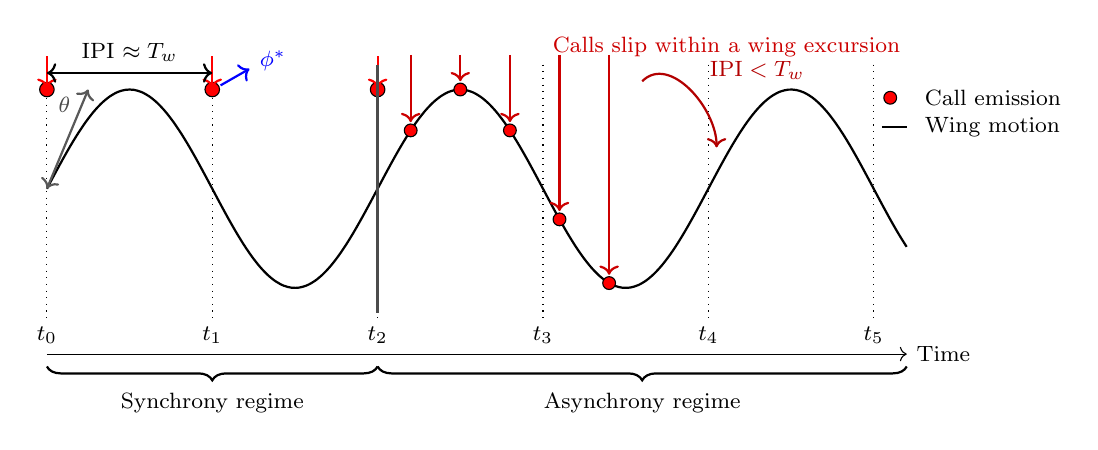
\begin{tikzpicture}[scale=1.05]
		
		% Parameters
		\def\A{1.2}         % Amplitude
		\def\T{2.0}         % Wingbeat period
		\def\Nsync{2}       % Number of sync cycles
		\def\Nasync{3.2}    % Number of async cycles after
		\def\dt{0.04}       % Step for smooth sine
		
		% Draw sine wave for wing excursion (sync + async, black)
		\draw[thick,black,domain=0:{(\Nsync+\Nasync)*\T},samples=110,smooth,variable=\t]
		plot ({\t},{\A*sin(180*\t/\T)});
		
		% Vertical lines for cycles
		\foreach \i in {0,...,5} {
			\draw[dotted] ({\i*\T},1.5) -- ({\i*\T},-1.6);
			\node[below] at ({\i*\T},-1.55) {\footnotesize $t_{\i}$};
		}
		
		% Synchrony calls (upstroke)
		\foreach \i in {0,1,2} {
			\pgfmathsetmacro\xcall{\i*\T}
			\draw[fill=red] (\xcall,\A) circle (2.5pt);
			\draw[->,red,thick] (\xcall,1.6) -- (\xcall,1.22);
			% phi* arrow for first
			\ifnum\i=1
			\draw[->,thick,blue] (2.1,1.25) -- (2.45,1.45);
			\node[above right=0.01cm,blue] at (2.45,1.3) {\footnotesize $\phi^*$};
			\fi
		}
		
		% Show synchrony regime bracket
		\draw [decorate,decoration={brace,amplitude=5pt,mirror},thick]
		(0,-2.15) -- ({\Nsync*\T},-2.15) node[midway,below=6pt] {\footnotesize Synchrony regime};
		
		% Draw IPI and Tw arrows (top)
		\draw[<->,thick] (0,1.4) -- (\T,1.4);
		\node[above] at (0.5*\T,1.42) {\footnotesize IPI $\approx T_w$};
		
		% Separator for asynchrony regime
		\draw[very thick,gray!60!black] ({\Nsync*\T},-1.5) -- ({\Nsync*\T},1.5);
		
		% Async calls (drift phase, not upstroke)
		\foreach \j [evaluate={\xcall=4.4+\j*0.6; \ycall=\A*sin(180*\xcall/\T);}] in {0,1,2,3,4} {
			\draw[fill=red] (\xcall,\ycall) circle (2.2pt);
			\draw[->,red!80!black,thick] (\xcall,1.62) -- (\xcall,\ycall+0.1);
		}
		\node[above right,red!80!black] at (6.0,1.48) {\footnotesize Calls slip within a wing excursion};
		
		% Asynchrony bracket
		\draw [decorate,decoration={brace,amplitude=5pt,mirror},thick]
		({\Nsync*\T},-2.15) -- ({(\Nsync+\Nasync)*\T},-2.15) node[midway,below=6pt] {\footnotesize Asynchrony regime};
		
		% Arrows
		\draw[->,thick,red!70!black] (7.2,1.3) to[out=45,in=90] (8.1,0.5);
		\node[above right,red!70!black] at (7.9,1.2) {\footnotesize $\mathrm{IPI} < T_w$};
		
		% Excursion angle (first cycle)
		\draw[<->,gray!70!black,thick] (0,0) -- (0.5,1.2);
		\node[above left,gray!60!black] at (0.4,0.8) {\footnotesize $\theta$};
		
		% Legend
		\draw[fill=red] (10.2,1.1) circle (2.2pt); \node[right] at (10.5,1.1) {\footnotesize Call emission};
		\draw[thick,black] (10.1,0.75) -- (10.4,0.75); \node[right] at (10.5,0.75) {\footnotesize Wing motion};
		
		% Axis
		\draw[->] (0,-2) -- ({(\Nsync+\Nasync)*\T+0},-2) node[right] {\footnotesize Time};
		
	\end{tikzpicture}
\end{document}